\documentclass[5pt]{article}
\usepackage{multicol,multirow}
\usepackage{graphicx} % Required for inserting images
\usepackage[margin=0.75cm]{geometry}
\usepackage{xcolor}
\usepackage{amsmath,esint}
\usepackage{mathtools}
\usepackage{relsize}
\usepackage{mathtools}
\usepackage{nccmath}
\usepackage[inline]{enumitem}
\usepackage{algpseudocode}

\usepackage{empheq}
\usepackage{amsfonts}

\usepackage{tkz-euclide}
\usepackage{tikz}

\definecolor{LightGray}{gray}{0.9}

\usepackage{minted}

\newenvironment{amatrix}[1]{%
  \left[\begin{array}{@{}*{#1}{c}|c@{}}
}{%
  \end{array}\right]
}

\DeclarePairedDelimiter\abs{\lvert}{\rvert}%
\DeclarePairedDelimiter\norm{\lVert\lVert}{\rVert\rVert}%

\makeatletter
\let\oldabs\abs
\def\abs{\@ifstar{\oldabs}{\oldabs*}}

\newcommand{\tr}[3]{
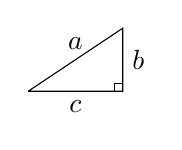
\begin{tikzpicture}[scale=0.40]
    \coordinate [] (A) at (-1.5cm,-1.cm);
    \coordinate [] (C) at (1.5cm,-1.0cm);
    \coordinate [] (B) at (1.5cm,1.0cm);
    \draw (A) -- node[above] {$a$} (B) -- node[right] {$b$} (C) -- node[below] {$c$} (A);
    \draw (1.25cm,-1.0cm) rectangle (1.5cm,-0.75cm);
\end{tikzpicture}
}


\begin{document}

\begin{center}
     \Large{\textbf{Science In The News}}\\
     \footnotesize{Class: SCIN 1030}\hfill\footnotesize{Maximilien Notz}
     \noindent\rule{20.2cm}{0.4pt}
\end{center}


\begin{multicols}{2}
\setcounter{secnumdepth}{0}

\subsection{Science}
\subsubsection{Epistemology}
    \begin{tabular}{ll}
        Epistemology    & Epistemology is the study of knowledge.\\ 
        A priori        & Knowledge of logical truths and of abstract\\
                        & claims (non-empirical).\\
        A posteriori    & Knowledge known by experience (empirical).\\
        Deduction       & \small{Theory$\rightarrow$Hypothesis$\rightarrow$Opservation$\rightarrow$Confirmation}\\
        Induction       & Opservation$\rightarrow$Pattern$\rightarrow$Hypothesis$\rightarrow$Theory\\
        Falsifiability  & Each scientist should attempt to disprove their\\
                        & theory to continually prove it.\\
    \end{tabular}

\subsubsection{Scientific Method Steps}
    \begin{enumerate}
        \item \textbf{Purpose:} State the Problem.
        \item \textbf{Research:} Research the Topic.
        \item \textbf{Hypothesis:} Formulate an Hypothesis.
        \item \textbf{Experiment:} Test your Hypothesis.
        \item \textbf{Analyze:} Analyze the experiment Data.
        \item \textbf{Conclusion:} Compare the hypothesis to the experiment result.
    \end{enumerate}

\subsubsection{Variables}
\begin{tabular}{ll}
    Variables                   & anything that can change during an\\
                                & experiment.\\
    Independent Variable        & The variable that is controlled or\\
                                & manipulated by the experimenter.\\
    Dependent Variable          & The variable that is measured by the\\   
                                & experimenter.\\
    Control Group               & The group that is not exposed to the\\
                                & independent variable.\\
\end{tabular}


\subsubsection{Common Pitfallsin Science and Science Communication}
\begin{tabular}{ll}
    Correlation         & A \textbf{correlation} between 2 variable does not\\
    vs Causation        & alway mean one \textbf{cause} the other.\\
    \hline
    Unsuported          & studies should be clear on the factes the study\\
    Conclusion          &  proves, and wich conclusion are unsuported.\\
    \hline
    Sample size         & In trial, the smaller a sample size, the lower\\
    problem             & the confidence in the result from that sample.\\
    \hline
    Unrepresantative    & If the sample is different from the population\\
    Sample used         & the confidence in the result from that sample.\\
    \hline
    No control          & Without a comparison group, we cannot\\
    group               & \small{separate intervention effects from other influences.}\\
    \hline
    No blind            & Subjects should not know if they if they are in\\
    testing used        & the test or control group.\\
    \hline
    Sensationalised     & Articles headline are commonly designed to\\
    headline            & entice viewers into reading it. This can\\
                        & over-simplifie findings or misrepresent them.\\
    \hline
    Misinterpreted      & News article can misinterpret the findings of\\
    results             & research for the sake of good story.\\
    \hline
    conflict of         & Research and data being misinterpret for\\
    Interest            & finantial or personal reasons.\\
    \hline
    Selective           & Selecting data from result wich support the\\
    reporting of data   & conclusion of the research, while ignoring those\\
                        & that do not.\\
    \hline
    Unreplicated        & Results should be replicable by independent\\
    results             & \small{research, and tested over wide ranges of conditions}.\\
    \hline
    Non-peer            & Other scientes appraise and critique studies,\\
    reviewed material   & before publication in a journal.\\
\end{tabular}


\subsection{Ethics}
\begin{tabular}{ll}
    Ethic       & Ethics is defined as the study of morality.\\
    Morality    & a system of rules for guiding human conduct.\\
    Directives  & rules that guide our actions.\\
    Micro-ethic & ethical issues at the level of individual decisions\\
                & and professional conduct.\\
    Macro-ethic & ethical issues at the societal or policy level\\
                & concerning the collective impacts of science and\\
                & technology.\\
\end{tabular}

\section{Critical analysis}


\end{multicols}
\end{document}
